\documentclass[tikz,border=5pt]{standalone}
\usetikzlibrary{calc}
\begin{document}
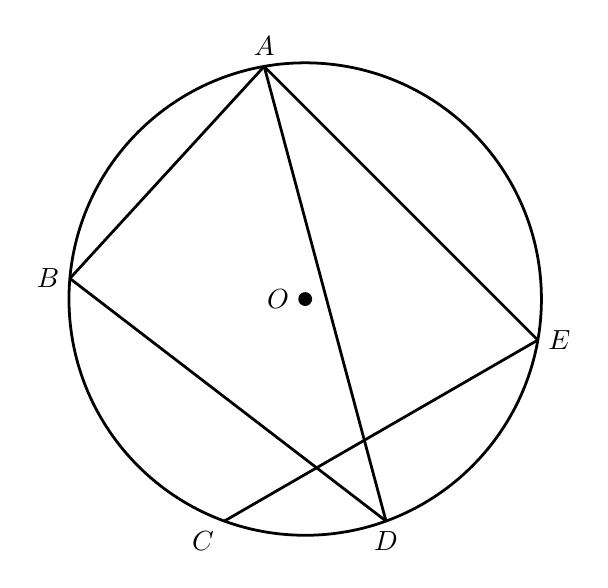
\begin{tikzpicture}[line width=1pt]
  % Circle
  \coordinate (O) at (0,0);
  \draw (O) circle (3cm);
  \fill (O) circle (2.5pt) node[left=2pt] {$O$};

  % Points on circle
  \coordinate (A) at (100:3cm);
  \coordinate (B) at (175:3cm);
  \coordinate (C) at (250:3cm);
  \coordinate (D) at (290:3cm);
  \coordinate (E) at (-10:3cm);

  % Segments
  \draw (A) -- (B);
  \draw (A) -- (E);
  \draw (B) -- (D);
  \draw (C) -- (E);
  \draw (A) -- (D);

  % Labels
  \node[above] at (A) {$A$};
  \node[left] at (B) {$B$};
  \node[below left] at (C) {$C$};
  \node[below] at (D) {$D$};
  \node[right] at (E) {$E$};
\end{tikzpicture}
\end{document}
